%% ReShift-STLA manuscript draft (Transportation Research Part C).
%% Built on the Elsevier elsarticle template (v3.4) supplied in this folder.
\documentclass[preprint,12pt,authoryear]{elsarticle}

\usepackage{amssymb}
\usepackage{amsmath}
\usepackage{bm}
\usepackage{booktabs}
\usepackage{array}
\usepackage{xcolor}
\usepackage{enumitem}
\usepackage{algorithm}
\usepackage{algorithmic}
\usepackage{tikz}
\usetikzlibrary{arrows.meta,positioning,fit,calc,backgrounds}
\usepackage[hidelinks]{hyperref}
\usepackage{lineno}

%% ---- drafting helpers (remove before submission) ----
\newcommand{\tbd}{\textcolor{red}{--}}
\newcommand{\todo}[1]{\textcolor{red}{[TODO: #1]}}
%% ---- notation ----
\newcommand{\X}{\mathbf{X}}
\newcommand{\Y}{\mathbf{Y}}
\newcommand{\M}{\mathbf{M}}
\newcommand{\B}{\mathbf{B}}
\newcommand{\Shift}{\mathbf{S}}
\newcommand{\Teach}{\mathcal{T}}
\newcommand{\Mem}{\mathcal{D}}
\newcommand{\R}{\mathbb{R}}

\journal{Transportation Research Part C: Emerging Technologies}

\begin{document}

\begin{frontmatter}

\title{ReShift: Restoring the forecast shift of sensor failures by coverage-allocated evolution retrieval, failure replay and counterfactual restoration}

%% TODO: replace the placeholder author block.
\author[aff1]{Author One\corref{cor1}}
\ead{author.one@example.org}
\author[aff1]{Author Two}
\cortext[cor1]{Corresponding author.}
\affiliation[aff1]{organization={Department, University},
            city={City},
            country={Country}}

\begin{abstract}
Network-wide traffic forecasters are trained on dense sensor histories but deployed on detector networks in which entries, whole sensors, time intervals, regions or travel directions routinely drop out. A forecaster that receives an incomplete history does not simply lose information; its output is displaced by a systematic, failure-specific bias that we call the \emph{restoration shift}, i.e.\ the difference between what the same model would predict from the complete history and what it predicts from the observed part. We propose ReShift, a correction framework that estimates and removes this shift, and instantiate it on a missing-aware spatio-temporal Transformer (STLAformer). ReShift combines three complementary evidence sources: (i) \emph{evolution retrieval}, which transfers the anchored future evolution of retrieved complete historical windows whose keys are aligned with incomplete queries by contrastive learning; (ii) \emph{failure replay}, which replays the query's own observation mask on similar complete historical windows through a frozen teacher and transfers their empirical restoration shifts; and (iii) \emph{counterfactual restoration}, a parametric estimate of the query's own restoration shift distilled from complete training histories. The three corrections are reranked per sensor and horizon against an explicit no-correction option, risk-gated, and combined by allocation gates that depend only on label-free observability descriptors such as local and neighbourhood coverage. All evidence comes from the training split and no query future or complete query history is used at inference. Experiments on the TraffiDent benchmark with five failure families and missing rates from 20\% to 90\% \todo{summarise headline results once the formal runs finish}.
\end{abstract}

\begin{highlights}
\item Sensor failures shift forecasts systematically; we model and remove this restoration shift.
\item Retrieved complete histories supply both future evolutions and replayed failure shifts.
\item A distilled counterfactual head estimates the query's own shift without complete inputs.
\item Coverage-conditioned gates allocate the three corrections per sensor and horizon.
\item Leakage-safe protocol: Train-only memory, no query futures, temporal-overlap exclusion.
\end{highlights}

\begin{keyword}
Traffic forecasting \sep Missing data \sep Sensor failure \sep Retrieval-augmented forecasting \sep Counterfactual restoration \sep Spatio-temporal Transformer
\end{keyword}

\end{frontmatter}

\linenumbers

\section{Introduction}
\label{sec:intro}

Short-term network-wide traffic forecasting underpins signal control, ramp metering, incident management and traveller information. Deep spatio-temporal models such as diffusion-convolutional recurrent networks \citep{li2018dcrnn}, spatio-temporal graph convolutional networks \citep{yu2018stgcn,wu2019graphwavenet,bai2020agcrn} and, more recently, spatio-temporal Transformers \citep{vaswani2017attention,stlaformer} have substantially improved accuracy on benchmark data. These models are almost always trained and evaluated on histories in which every detector reports every interval. In operation this assumption is routinely violated: loop detectors fail individually, communication links drop whole corridors, maintenance removes sensors for hours, and power or data-pipeline incidents remove entire regions or one travel direction at once \citep{cui2020missing,chen2019bayesian}.

Two families of remedies exist. \emph{Impute-then-forecast} pipelines first reconstruct the missing history with a dedicated model \citep{cao2018brits,cini2022grin,tashiro2021csdi,chen2019bayesian} and then run a standard forecaster. \emph{Direct} approaches feed the incomplete history together with its mask to a forecaster that has been made missing-aware \citep{che2018grud,tang2020joint,cui2020missing}. Both families treat missingness as a loss of input information that has to be compensated inside the network. What they do not model explicitly is the consequence of missingness on the \emph{output} of a given forecaster. For a fixed model, removing inputs displaces the forecast in a systematic way that depends on which entries are missing, where they are in the network, and how far ahead one predicts. We call this displacement the \emph{restoration shift}: the difference between the forecast the same model would make from the complete history and the forecast it makes from the observed part. If the restoration shift could be estimated at deployment time, it could simply be added back.

Estimating the restoration shift is hard because, by definition, the complete history of the query is not available. This paper argues that two kinds of evidence are nevertheless available and that they are complementary.
\emph{Historical evidence} is plentiful: a traffic network repeats its daily and weekly patterns, so complete historical windows that resemble the observed part of the query are informative about how the query will evolve, and, crucially, one can artificially impose the query's own failure pattern on those windows and observe how the forecaster reacts.
\emph{Parametric evidence} is available in training: for training windows both the incomplete and the complete history exist, so a model can be taught to predict the restoration shift directly from the incomplete input.
We expect the value of each source to depend on how much of the neighbourhood is still observed. When most of the neighbourhood reports, the observed part of the query identifies good historical analogues and their future evolution transfers well. When most of the neighbourhood is dark, analogues become ambiguous, but the forecaster's reaction to the failure pattern itself, which is what replay and counterfactual restoration capture, becomes the dominant source of error.

Building on this view we propose \textbf{ReShift}, a correction framework placed on top of a missing-aware STLAformer backbone. Its contributions are:
\begin{enumerate}[leftmargin=*,label=(\arabic*)]
\item We formalise the \emph{restoration shift} of a forecaster under an observation mask and use a frozen copy of the pretrained forecaster as a teacher that defines it on training data (Section~\ref{sec:problem}).
\item We introduce \emph{evolution retrieval}, which transfers anchored future evolutions of retrieved complete training windows; retrieval keys of incomplete queries are aligned with those of complete windows by a contrastive objective with a momentum-updated memory encoder (Section~\ref{sec:evolution}).
\item We introduce \emph{failure replay}, which imposes the query's own mask on complete training windows that resemble its observed part and transfers their teacher restoration shifts, i.e.\ empirical evidence about how this particular failure pattern displaces the forecast (Section~\ref{sec:replay}).
\item We add a \emph{counterfactual restoration} head that predicts the query's own restoration shift and is distilled from the teacher on complete training histories (Section~\ref{sec:cf}).
\item We combine the three corrections with \emph{coverage-conditioned allocation gates} that see only label-free observability descriptors, after per-sensor, per-horizon reranking against an explicit no-correction option and risk gating (Section~\ref{sec:allocation}).
\item We evaluate under a leakage-safe protocol with five failure families and missing rates from 20\% to 90\%, independent ablations and in-checkpoint interventions that test whether each component uses its evidence as intended (Sections~\ref{sec:experiments}--\ref{sec:results}).
\end{enumerate}

The remainder of the paper is organised as follows. Section~\ref{sec:related} reviews related work. Section~\ref{sec:problem} defines the problem and the restoration shift. Section~\ref{sec:method} presents ReShift. Section~\ref{sec:experiments} describes the experimental protocol, Section~\ref{sec:results} reports results, Section~\ref{sec:discussion} discusses limitations and Section~\ref{sec:conclusion} concludes.

\section{Related work}
\label{sec:related}

\paragraph{Spatio-temporal traffic forecasting}
Graph-based recurrent and convolutional models \citep{li2018dcrnn,yu2018stgcn,wu2019graphwavenet,bai2020agcrn} couple temporal sequence modelling with spatial message passing over a road or learned graph. Attention-based architectures \citep{vaswani2017attention} have since been adapted to spatio-temporal data; ReShift uses STLAformer \citep{stlaformer} as its backbone but does not depend on its internals beyond a latent representation and the forecast. Classical non-parametric forecasting based on nearest historical neighbours \citep{davis1991nonparametric,smith1997traffic} is an early form of retrieval: future traffic is predicted from the futures of similar past states. ReShift revisits this idea inside a deep forecaster and under missing inputs.

\paragraph{Forecasting with missing observations}
Imputation methods reconstruct missing entries using recurrent dynamics \citep{che2018grud,cao2018brits}, graph neural networks \citep{cini2022grin}, low-rank tensor or matrix structure \citep{chen2019bayesian} or conditional diffusion models \citep{tashiro2021csdi}. Their reconstructions can be passed to any forecaster, but reconstruction error propagates and the imputer is not trained for the downstream forecasting loss. Direct approaches make the forecaster aware of the mask, for example through decay mechanisms \citep{che2018grud}, joint local and global modelling \citep{tang2020joint} or masking-aware recurrent architectures for network-wide traffic \citep{cui2020missing}. ReShift is complementary: it starts from such a missing-aware forecaster and estimates what remains of the failure-induced error in output space.

\paragraph{Retrieval-augmented prediction}
Retrieval augmentation conditions a parametric model on examples fetched from a datastore, as in nearest-neighbour language models \citep{khandelwal2020knnlm} and retrieval-augmented generation \citep{lewis2020rag}. For time series, retrieval is attractive because recurrent daily and weekly patterns make the training set an informative memory. Two difficulties are specific to the incomplete setting: queries and memory items are described under different observation conditions, which we address with contrastive key alignment \citep{oord2018cpc} and a momentum memory encoder \citep{he2020moco}; and retrieved futures may be wrong for the query, which we address with per-element reranking against a no-correction option and risk gating.

\paragraph{Counterfactual targets and distillation}
Using a fixed model to produce training targets for another model is the essence of knowledge distillation \citep{hinton2015distilling}. ReShift uses a frozen copy of the pretrained forecaster as a teacher, but distils a quantity that is not a prediction of the data: the teacher's own counterfactual change of output when the missing entries are restored. We are not aware of work that treats this restoration shift as the object of estimation and estimates it jointly from retrieved, replayed and parametric evidence for traffic forecasting \todo{confirm with a systematic literature search}.

\section{Problem formulation}
\label{sec:problem}

\paragraph{Data and observation masks}
Consider a detector network with $N$ sensors sampled every 5 minutes. A forecasting window consists of a history $\X\in\R^{L\times N}$ of $L$ steps and a future $\Y\in\R^{P\times N}$ of $P$ steps of the target variable (speed or flow), together with time-of-day and day-of-week indices. At deployment only a subset of the history is observed. We write the observation mask as $\M\in\{0,1\}^{L\times N}$, the observed history as $\X\odot\M$, and the forecasting task as
\begin{equation}
\widehat{\Y}=F\big(\X\odot\M,\ \M\big)\approx\Y .
\label{eq:task}
\end{equation}
Masks follow structured failure families (Section~\ref{sec:data}): random entries, whole-sensor outages, temporal outages, regional outages and directional outages. The \emph{severity} of a mask is the fraction of history entries it removes.

\paragraph{Training memory}
The training split provides, for every window, the complete history $\X$, the future $\Y$ and one benchmark mask $\M$. We denote by $\Mem=\{(\X_j,\Y_j,\tau_j)\}_{j=1}^{|\Mem|}$ the set of complete training windows with start times $\tau_j$. $\Mem$ is the only source of retrieved evidence at training, validation and test time. A memory item is \emph{legal} for a query starting at $\tau$ if the two windows do not overlap, $|\tau_j-\tau|\geq L+P$.

\paragraph{Restoration shift}
Let $\Teach$ be a forecaster that accepts an incomplete history and its mask. The restoration shift of a window $\X$ under mask $\M$ is
\begin{equation}
\Shift_{\Teach}(\X,\M)=\Teach(\X,\mathbf{1})-\Teach(\X\odot\M,\M),
\label{eq:shift}
\end{equation}
i.e.\ the change of the forecast that restoring the missing entries would cause. It decomposes the error of the incomplete forecast as
\begin{equation}
\Y-\Teach(\X\odot\M,\M)=\underbrace{\Shift_{\Teach}(\X,\M)}_{\text{failure-induced}}+\underbrace{\big(\Y-\Teach(\X,\mathbf{1})\big)}_{\text{complete-history error}} .
\label{eq:decomp}
\end{equation}
The first term is caused by the failure and vanishes when nothing is missing; the second term is the error the forecaster would make anyway. In ReShift, $\Teach$ is a frozen copy of the pretrained backbone. Equation~\eqref{eq:shift} can be evaluated whenever a complete history is known, which is the case for every item in $\Mem$ and for every training query, but never for a validation or test query.

\paragraph{Causality constraints}
At inference, the model may use only $\X\odot\M$, $\M$, calendar indices, the query start time (to enforce legality) and $\Mem$. It may not use the query future, the complete query history or any validation or test window as evidence. Labels are used only in training losses and for evaluation.

\section{Methodology}
\label{sec:method}

\subsection{Overview}
ReShift (Fig.~\ref{fig:overview}) predicts
\begin{equation}
\widehat{\Y}=\B+g_E\odot\mathbf{C}_E+g_R\odot\mathbf{C}_R+g_S\odot\mathbf{C}_S ,
\label{eq:reshift}
\end{equation}
where $\B$ is the forecast of a missing-aware backbone, $\mathbf{C}_E$, $\mathbf{C}_R$ and $\mathbf{C}_S$ are the evolution-retrieval, failure-replay and counterfactual-restoration corrections, and $g_E,g_R,g_S\in(0,1)^{P\times N}$ are allocation gates. All quantities are per sensor and per horizon. Each correction is bounded, $|\mathbf{C}|\le\Delta$ in normalised units ($\Delta=3$), and each is designed so that the model can fall back to $\B$ when the evidence is unreliable.

\begin{figure}[t]
\centering
\resizebox{\textwidth}{!}{%
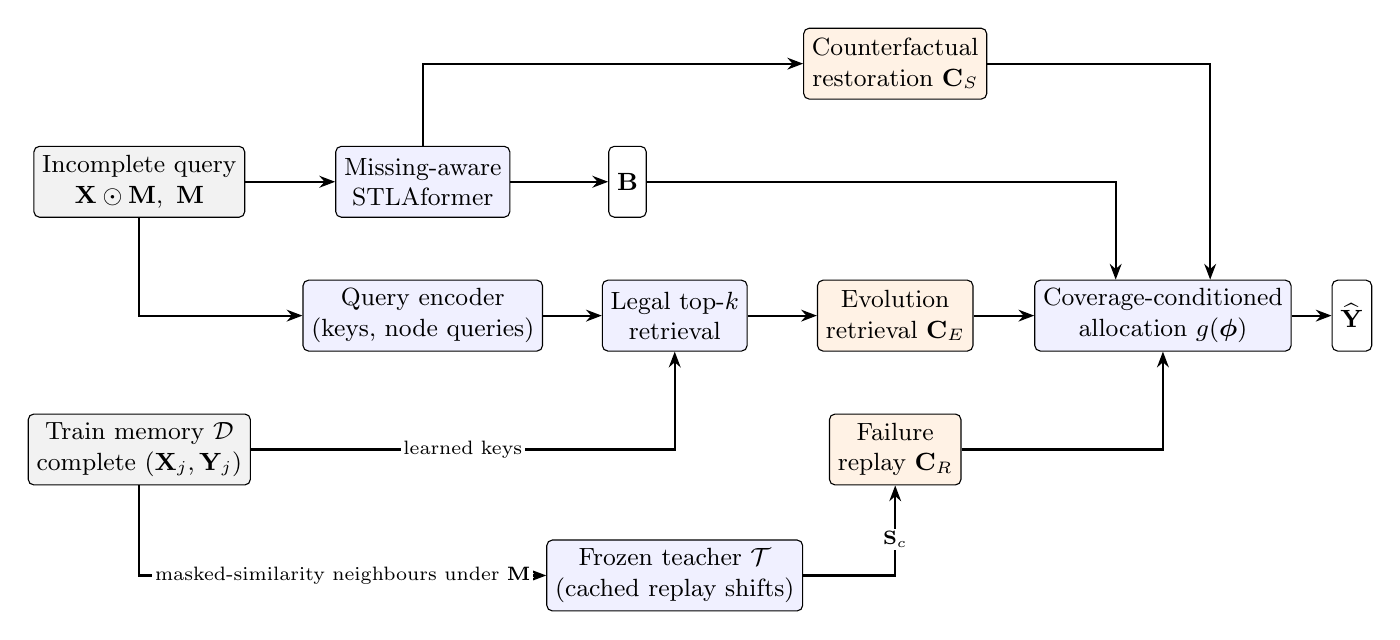
\begin{tikzpicture}[
  font=\small,
  box/.style={draw, rounded corners=2pt, align=center, minimum height=9mm, inner sep=3pt, fill=white},
  data/.style={box, fill=gray!10}, mod/.style={box, fill=blue!6}, corr/.style={box, fill=orange!10},
  arr/.style={-{Stealth[length=2mm]}, thick}, lab/.style={font=\scriptsize, fill=white, inner sep=1pt}]
\node[data] (q)   at (0,0)     {Incomplete query\\$\X\odot\M,\ \M$};
\node[mod]  (bb)  at (3.6,0)   {Missing-aware\\STLAformer};
\node[box]  (B)   at (6.2,0)   {$\B$};
\node[corr] (cf)  at (9.6,1.5) {Counterfactual\\restoration $\mathbf{C}_S$};
\node[mod]  (enc) at (3.6,-1.7){Query encoder\\(keys, node queries)};
\node[mod]  (ret) at (6.8,-1.7){Legal top-$k$\\retrieval};
\node[corr] (evo) at (9.6,-1.7){Evolution\\retrieval $\mathbf{C}_E$};
\node[data] (mem) at (0,-3.4)  {Train memory $\Mem$\\complete $(\X_j,\Y_j)$};
\node[mod]  (tch) at (6.8,-5.0){Frozen teacher $\Teach$\\(cached replay shifts)};
\node[corr] (rep) at (9.6,-3.4){Failure\\replay $\mathbf{C}_R$};
\node[mod]  (al)  at (13.0,-1.7){Coverage-conditioned\\allocation $g(\bm\phi)$};
\node[box]  (out) at (15.4,-1.7){$\widehat{\Y}$};
\draw[arr] (q) -- (bb); \draw[arr] (bb) -- (B);
\draw[arr] (q.south) |- (enc.west); \draw[arr] (enc) -- (ret); \draw[arr] (ret) -- (evo);
\draw[arr] (mem.east) -| node[lab, pos=0.25]{learned keys} (ret.south);
\draw[arr] (mem.south) |- node[lab, pos=0.75]{masked-similarity neighbours under $\M$} (tch.west);
\draw[arr] (tch.east) -| node[lab, pos=0.7]{$\Shift_c$} (rep.south);
\draw[arr] (bb.north) |- (cf.west);
\draw[arr] (cf.east) -| ([xshift=6mm]al.north);
\draw[arr] (B.east) -| ([xshift=-6mm]al.north);
\draw[arr] (evo) -- (al); \draw[arr] (rep.east) -| (al.south);
\draw[arr] (al) -- (out);
\end{tikzpicture}}
\caption{Overview of ReShift. The backbone forecast $\B$ is corrected by three bounded, risk-gated corrections that are combined by allocation gates depending only on observability descriptors. Replay shifts and counterfactual targets are computed once with the frozen teacher and cached; memory keys are produced by a momentum (EMA) copy of the query encoder.}
\label{fig:overview}
\end{figure}

\subsection{Missing-aware backbone}
\label{sec:backbone}
The backbone is a pretrained STLAformer \citep{stlaformer} whose input embedding is augmented with an observation-pattern embedding $\mathrm{MLP}([m_{\ell n},\bar m_{\cdot n},\bar m_{\ell\cdot},a_{\ell n}])$ of the mask entry, the node's coverage over the history, the step's coverage over the network and the normalised time since the node was last observed. The last layer of this embedding is initialised at zero, so at initialisation the backbone reproduces the pretrained model exactly. The backbone is fine-tuned progressively: during a warm-up phase only the new modules are trained, then the last two spatio-temporal attention layers and the output projection are unfrozen, and finally the whole backbone. It produces the forecast $\B=f_\theta(\X\odot\M,\M)$ and a node representation $\mathbf{z}_n$ (the history average of the last hidden layer). A frozen copy of the \emph{unchanged} pretrained model serves as the teacher $\Teach$ in Eq.~\eqref{eq:shift}.

\subsection{Query encoder and legal retrieval}
\label{sec:retrieval}
A light observation-state encoder describes each node by (a) an MLP over its history of values, mask, missing age and time of week, and (b) a summary of observed mean, standard deviation, last observed value, coverage and last missing age plus a learned node embedding. Spatial context is aggregated by multi-head attention over the $K=8$ neighbours of a Train-only statistical graph, obtained from positive, lag-aware correlations of complete training histories; neighbours without observations are masked out, so a fully unobserved node is still described by its observed neighbours. Coverage-weighted pooling over nodes yields two normalised global keys, a temporal key $\mathbf{k}^T$ and a spatial key $\mathbf{k}^S$, and the encoder also outputs a node query $\mathbf{q}_n$.

The same architecture, updated as an exponential moving average of the query encoder \citep{he2020moco}, encodes every complete window in $\Mem$. For each query we retrieve the top-$k$ legal items by cosine similarity for each key ($k=6$), giving $C=2k$ candidates with global scores $s_c$. Memory keys are re-encoded every few epochs and before every validation pass.

\subsection{Evolution retrieval}
\label{sec:evolution}
A candidate's future cannot be copied directly, because its level may differ from the query. Instead we transfer its \emph{evolution} relative to the last time the query was observed. For node $n$ let $\ell^\ast_n$ be the last observed history step and $a_n$ the anchor: the last observed value of the node; if the node is never observed, the mean last observed value of its observed graph neighbours; if none exists, the first backbone step. The candidate forecast is
\begin{equation}
\widehat{\Y}_c[p,n]=a_n+\Y_c[p,n]-\X_c[\ell^\ast_n,n] .
\end{equation}
For a node with no observation at all we instead transfer the candidate's innovation with respect to a Train-only hour-of-week mean, $\widehat{\Y}_c=\B+\Y_c-\bm\mu_{b(c)}$, which also allows a non-zero first-step correction. The candidate residual is $\mathbf{r}_c=\widehat{\Y}_c-\B$.

Not every candidate is useful for every sensor and horizon. A scoring network maps element-wise features (backbone forecast, candidate forecast, residual, evolution increment, observed-history distance, global score, node-level similarity between $\mathbf{q}_n$ and the memory node query, local and neighbour coverage, node context and horizon embedding) to a logit $\lambda_c[p,n]$, to which $s_c$ is added. A separate network produces a \emph{no-correction} logit $\lambda_0[p,n]$ from the context alone. With weights $w=\mathrm{softmax}(\lambda_0,\lambda_1,\dots,\lambda_C)$ over the $C+1$ options, the aggregated evidence and its dispersion are
\begin{equation}
\mathbf{e}_E=\sum_{c=1}^C w_c\,\mathbf{r}_c,\qquad \bm\sigma_E=\Big(\sum_c w_c(\mathbf{r}_c-\mathbf{e}_E)^2\Big)^{1/2}.
\end{equation}
A risk gate $\rho_E=\mathrm{sigmoid}(\mathrm{MLP}([\text{context},\bm\sigma_E,1-w_0]))$ estimates the probability that applying the evidence improves the backbone, and
\begin{equation}
\mathbf{C}_E=\rho_E\odot\Delta\tanh(\mathbf{e}_E/\Delta).
\end{equation}

\subsection{Failure replay}
\label{sec:replay}
Evolution retrieval answers ``how did similar situations evolve?''. Failure replay answers a different question: ``how does \emph{this} failure pattern displace the forecast in similar situations?''. For each query we select $R=4$ legal training windows by cosine similarity computed only over the query's observed entries,
\begin{equation}
\kappa(\X\odot\M,\X_j)=\frac{\langle \X\odot\M,\ \X_j\odot\M\rangle}{\lVert\X\odot\M\rVert\,\lVert\X_j\odot\M\rVert},
\end{equation}
impose the query's mask on their complete histories, and compute their teacher restoration shifts
\begin{equation}
\Shift_c=\Teach(\X_c,\mathbf{1})-\Teach(\X_c\odot\M,\M) .
\end{equation}
Because $\Shift_c$ is measured under exactly the query's failure pattern, it carries information about the failure-induced error term of Eq.~\eqref{eq:decomp} that the candidate's future does not. The replay shortlist is deliberately label-free and independent of the learned retrieval keys. As a consequence, and because benchmark masks are fixed per window, the shifts of every training, validation and test query can be computed once with the frozen teacher and cached; training then requires no teacher pass at all. For training queries the shortlist additionally excludes windows within one day of the query, so that training neighbours are not systematically closer in time than test neighbours. The shifts are reranked against a no-correction option, aggregated and risk-gated as in Section~\ref{sec:evolution} (element features $\Shift_c$ and $|\Shift_c|$; candidate features the horizon-average of $|\Shift_c|$ and $\kappa$; the same context features), giving $\mathbf{C}_R$.

\subsection{Counterfactual restoration}
\label{sec:cf}
The third correction estimates the query's own restoration shift parametrically. A head $h_\psi$ maps the backbone forecast, observability descriptors, the projected node representation $\mathbf{z}_n$, the projected node query $\mathbf{q}_n$ and a horizon embedding to
\begin{equation}
\mathbf{C}_S=\Delta\tanh\big(h_\psi(\cdot)/\Delta\big).
\end{equation}
For training queries the complete history is known, so the target $\Shift_\Teach(\X,\M)$ of Eq.~\eqref{eq:shift} can be computed; the head is trained with a Huber loss towards it. Its last layer is initialised at zero. At inference the head only sees the incomplete input.

\subsection{Coverage-conditioned allocation}
\label{sec:allocation}
The three corrections are expected to be useful under different observability conditions. We therefore make the allocation gates depend only on label-free observability descriptors,
\begin{equation}
(g_E,g_R,g_S)=\mathrm{sigmoid}\big(\mathrm{MLP}(\bm\phi)\big),\qquad
\bm\phi[p,n]=\big(\bar m_{\cdot n},\ \bar m_{\mathcal N(n)},\ a_{Ln},\ \bar m,\ \mathbf{h}_p\big),
\end{equation}
namely the node's coverage, the coverage of its graph neighbours, its time since the last observation, the overall coverage of the query and a horizon embedding. Restricting $\bm\phi$ to observability has two purposes: it keeps the allocation interpretable (the learned gates can be plotted against coverage) and it prevents the allocation from re-learning the reliability that the risk gates already estimate from the evidence. We compare this choice with two alternatives: summation ($g\equiv1$) and a learned allocation that additionally sees correction magnitudes, no-correction weights and dispersions. The output layer is initialised with biases $(1.5,1.5,0)$, i.e.\ the counterfactual correction starts at half weight and with zero output.

\subsection{Training objective}
\label{sec:loss}
Let $\mathcal{L}_{\mathrm{MAE}}$ and $\mathcal{L}_{\mathrm{RMSE}}$ be the errors of $\widehat{\Y}$ in raw units on valid future entries. The objective is
\begin{equation}
\begin{aligned}
\mathcal{L}={}&\mathcal{L}_{\mathrm{MAE}}+\lambda_1\mathcal{L}_{\mathrm{RMSE}}+\lambda_2\mathcal{L}_{\mathrm{MAE}}(\B)
+\lambda_3\!\!\sum_{b\in\{E,R\}}\!\!\mathcal{L}^{b}_{\mathrm{rank}}+\lambda_4\!\!\sum_{b\in\{E,R\}}\!\!\mathcal{L}^{b}_{\mathrm{risk}}\\
&+\lambda_5\,\mathrm{Huber}\big(\mathbf{C}_S,\Shift_\Teach(\X,\M)\big)+\lambda_6\mathcal{L}_{\mathrm{align}} .
\end{aligned}
\end{equation}
The \emph{backbone-preservation} term keeps $\B$ accurate on its own, so that corrections remain corrections. For the \emph{ranking} terms, the utility of candidate $c$ at an element is $u_c=|\B-\Y|-|\B+\mathbf{r}_c-\Y|$ (normalised units); candidates with $u_c>\epsilon$ are pushed above the no-correction logit and those with $u_c<-\epsilon$ below it with a softplus loss ($\epsilon=0.02$). The \emph{risk} terms are binary cross-entropies whose targets indicate whether the ungated correction improves the backbone by more than $\epsilon$. The \emph{alignment} term is an InfoNCE loss \citep{oord2018cpc} between the keys of each incomplete training query and the memory-encoder keys of its own complete window, with temporally overlapping windows excluded from the negatives. We use $(\lambda_1,\dots,\lambda_6)=(0.05,0.15,0.05,0.03,0.10,0.10)$.

\begin{algorithm}[t]
\caption{One ReShift training step}
\label{alg:train}
\begin{algorithmic}[1]
\REQUIRE batch of incomplete training queries $(\X\odot\M,\M,\Y)$; memory $\Mem$; memory index; cached replay shifts and counterfactual targets
\STATE $\B,\mathbf{z}\leftarrow f_\theta(\X\odot\M,\M)$;\quad keys, node queries $\leftarrow$ query encoder
\STATE retrieve $C=2k$ legal candidates from $\Mem$ by temporal and spatial keys
\STATE $\mathbf{C}_E\leftarrow$ anchored evolutions, reranked against no-correction, risk-gated
\STATE look up the cached replay shifts $\Shift_c$ of the query's $R$ masked-similarity neighbours
\STATE $\mathbf{C}_R\leftarrow$ replayed shifts, reranked against no-correction, risk-gated
\STATE $\mathbf{C}_S\leftarrow h_\psi(\cdot)$;\quad cached target $\Shift_\Teach(\X,\M)$ from the query's complete Train history
\STATE $g\leftarrow\mathrm{sigmoid}(\mathrm{MLP}(\bm\phi))$;\quad $\widehat{\Y}\leftarrow\B+\sum_b g_b\odot\mathbf{C}_b$
\STATE update all trainable parameters with $\nabla\mathcal{L}$; update the memory encoder by EMA
\end{algorithmic}
\end{algorithm}

\subsection{Leakage safeguards and cost}
\label{sec:leakage}
The forward pass receives only the observed history, the mask, calendar indices and the query start time, which is used solely to exclude overlapping memory items. Every future used as evidence belongs to the training split, and the counterfactual target is constructed outside the model and only for training queries. A unit test perturbs all labels of a batch and verifies that predictions are unchanged. Per query, inference costs one backbone pass, two similarity searches over $|\Mem|$ normalised keys, encoding and scoring of $C$ candidates, and, for replay, one masked similarity search and $R$ teacher passes; the replay part is computed once per window and cached, so it is paid once and shared by all training runs. The candidate scorers are factorised: since their first layer is linear, element-, candidate- and context-level features are projected separately and only summed on the $[C,P,N]$ grid, which avoids materialising the concatenated feature tensor. \todo{Report measured training time per epoch, inference latency and GPU memory.}

\section{Experimental design}
\label{sec:experiments}

\subsection{Data and failure protocol}
\label{sec:data}
We use network 06 of the TraffiDent benchmark \citep{traffident}, which contains $N=388$ detectors sampled at 5-minute resolution. \todo{Describe the region, period and raw data source of TraffiDent Net 06; add the other networks if they are included.} We forecast speed and flow separately, with history and horizon $L=P=12$ steps (one hour each). Windows are split chronologically into training, validation and test sets \todo{state the split boundaries}. The training split contains 50{,}000 windows and the validation split 5{,}000 windows; each test severity contains 5{,}000 windows.

Missingness is imposed by a fixed benchmark protocol with five failure families: \emph{random entries}, \emph{sensor outages} (all steps of a set of sensors), \emph{temporal outages} (all sensors over an interval), \emph{regional outages} (a spatially contiguous group of sensors) and \emph{directional outages} (sensors of one travel direction). Training and validation masks have severity 40\%. Test masks are generated at severities 20\%, 40\%, 60\% and 90\%, so that 60\% and 90\% are more severe than anything seen during training. All masks are fixed and shared by all methods.

\subsection{Compared models}
\begin{itemize}[leftmargin=*]
\item \textbf{STLAformer}: the pretrained backbone applied to zero-filled incomplete histories without fine-tuning.
\item \textbf{Missing-aware STLAformer}: the backbone of Section~\ref{sec:backbone} fine-tuned with the same schedule and the forecasting and preservation losses, but without any correction branch (ablation \texttt{base\_only}).
\item \todo{Impute-then-forecast baselines, e.g.\ a graph imputer \citep{cini2022grin} or a low-rank tensor imputer \citep{chen2019bayesian} followed by STLAformer.}
\item \todo{Direct missing-aware forecasters, e.g.\ \citet{cui2020missing}, \citet{tang2020joint}.}
\item \textbf{ReShift} (ours).
\end{itemize}

\subsection{Ablations and interventions}
\emph{Independently trained ablations} remove one component and retrain from the same initialisation and schedule: no evolution retrieval (\texttt{no\_evolution}), no failure replay (\texttt{no\_replay}), no counterfactual restoration (\texttt{no\_cf}), summation instead of allocation (\texttt{fusion\_sum}), allocation with evidence statistics (\texttt{fusion\_learned}), no contrastive alignment (\texttt{no\_alignment}) and no risk gates (\texttt{no\_risk}).
\emph{In-checkpoint interventions} change a single input of the trained full model at test time: replacing retrieved windows by unrelated but legal training windows while keeping their scores (\texttt{wrong\_evidence}), zeroing one allocation gate (\texttt{drop\_evolution}, \texttt{drop\_replay}, \texttt{drop\_cf}), and returning the backbone forecast only (\texttt{base}). Interventions test whether the trained model actually relies on correct evidence; ablations test whether a component is needed when the rest of the model can adapt.

\subsection{Metrics}
We report MAE and RMSE in raw units over valid future entries, and MAPE over entries with $|y|>1$. Results are given per severity and as the macro average over the four severities. We additionally report errors on directly masked sensors, per failure family and at horizons 3, 6 and 12. \todo{Number of seeds; report mean $\pm$ standard deviation over seeds and a paired block-bootstrap test.}

\subsection{Implementation}
The model is implemented in PyTorch and trained on one NVIDIA V100 (32\,GB) with mixed precision. We use AdamW with learning rates $8\times10^{-4}$ for new modules and $5\times10^{-5}$ for the backbone, weight decay $10^{-4}$, batch size 64 and gradient clipping at 5. The warm-up phase lasts 8 epochs, partial fine-tuning lasts until epoch 30, and training stops after at most 60 epochs or 15 epochs without validation improvement in the final phase. The checkpoint with the lowest validation MAE is evaluated once on the test sets. Retrieval uses $k=6$ candidates per key, replay uses $R=4$ candidates, the memory encoder momentum is 0.995 and the memory index is refreshed every 5 epochs. \todo{Hyper-parameter sensitivity for $k$, $R$ and the allocation inputs.}

\section{Results}
\label{sec:results}

\todo{All numbers in this section are placeholders (\tbd) to be filled from the formal runs. Do not interpret any table before then.}

\subsection{Overall accuracy}
Table~\ref{tab:main} reports MAE and RMSE per severity. \todo{Describe the main result: macro-average improvement over the pretrained and the missing-aware backbone, and how the improvement changes with severity.}

\begin{table}[t]
\centering
\caption{Test MAE / RMSE on TraffiDent Net 06 by missing severity. Best in bold.}
\label{tab:main}
\small
\setlength{\tabcolsep}{4pt}
\begin{tabular}{llccccc}
\toprule
Target & Model & 20\% & 40\% & 60\% & 90\% & Macro \\
\midrule
Speed & STLAformer & \tbd/\tbd & \tbd/\tbd & \tbd/\tbd & \tbd/\tbd & \tbd/\tbd \\
 & Missing-aware STLAformer & \tbd/\tbd & \tbd/\tbd & \tbd/\tbd & \tbd/\tbd & \tbd/\tbd \\
 & \todo{baselines} & \tbd/\tbd & \tbd/\tbd & \tbd/\tbd & \tbd/\tbd & \tbd/\tbd \\
 & ReShift & \tbd/\tbd & \tbd/\tbd & \tbd/\tbd & \tbd/\tbd & \tbd/\tbd \\
\midrule
Flow & STLAformer & \tbd/\tbd & \tbd/\tbd & \tbd/\tbd & \tbd/\tbd & \tbd/\tbd \\
 & Missing-aware STLAformer & \tbd/\tbd & \tbd/\tbd & \tbd/\tbd & \tbd/\tbd & \tbd/\tbd \\
 & \todo{baselines} & \tbd/\tbd & \tbd/\tbd & \tbd/\tbd & \tbd/\tbd & \tbd/\tbd \\
 & ReShift & \tbd/\tbd & \tbd/\tbd & \tbd/\tbd & \tbd/\tbd & \tbd/\tbd \\
\bottomrule
\end{tabular}
\end{table}

\subsection{Contribution of each component}
Table~\ref{tab:ablation} reports the independently trained ablations. The design of Section~\ref{sec:method} leads to three testable expectations: (E1) removing evolution retrieval hurts mainly at low and moderate severity, where the observed neighbourhood still identifies good analogues; (E2) removing failure replay or counterfactual restoration hurts mainly at high severity, where the failure-induced term of Eq.~\eqref{eq:decomp} dominates; (E3) coverage-conditioned allocation is at least as accurate as summation and as evidence-conditioned allocation. \todo{Report whether E1--E3 hold.}

\begin{table}[t]
\centering
\caption{Independently trained ablations: change of test MAE relative to the full model (\%, positive = worse).}
\label{tab:ablation}
\footnotesize
\setlength{\tabcolsep}{3pt}
\begin{tabular}{lcccccccccc}
\toprule
 & \multicolumn{5}{c}{Speed} & \multicolumn{5}{c}{Flow}\\
\cmidrule(lr){2-6}\cmidrule(lr){7-11}
Variant & 20 & 40 & 60 & 90 & Macro & 20 & 40 & 60 & 90 & Macro\\
\midrule
Missing-aware backbone only & \tbd & \tbd & \tbd & \tbd & \tbd & \tbd & \tbd & \tbd & \tbd & \tbd\\
w/o evolution retrieval & \tbd & \tbd & \tbd & \tbd & \tbd & \tbd & \tbd & \tbd & \tbd & \tbd\\
w/o failure replay & \tbd & \tbd & \tbd & \tbd & \tbd & \tbd & \tbd & \tbd & \tbd & \tbd\\
w/o counterfactual restoration & \tbd & \tbd & \tbd & \tbd & \tbd & \tbd & \tbd & \tbd & \tbd & \tbd\\
Summation ($g\equiv1$) & \tbd & \tbd & \tbd & \tbd & \tbd & \tbd & \tbd & \tbd & \tbd & \tbd\\
Evidence-conditioned allocation & \tbd & \tbd & \tbd & \tbd & \tbd & \tbd & \tbd & \tbd & \tbd & \tbd\\
w/o contrastive alignment & \tbd & \tbd & \tbd & \tbd & \tbd & \tbd & \tbd & \tbd & \tbd & \tbd\\
w/o risk gates & \tbd & \tbd & \tbd & \tbd & \tbd & \tbd & \tbd & \tbd & \tbd & \tbd\\
\bottomrule
\end{tabular}
\end{table}

\subsection{Does the model use its evidence?}
Table~\ref{tab:audit} applies the in-checkpoint interventions. If evolution retrieval and failure replay exploit the content of the retrieved windows, replacing them with unrelated legal windows should remove most of their benefit, and dropping a branch should cost accuracy mainly in the severity range where that branch is expected to help. \todo{Interpret.}

\begin{table}[t]
\centering
\caption{In-checkpoint interventions on the trained full model: change of test MAE (\%, positive = worse).}
\label{tab:audit}
\small
\begin{tabular}{llccccc}
\toprule
Target & Intervention & 20\% & 40\% & 60\% & 90\% & Macro\\
\midrule
Speed & wrong evidence & \tbd & \tbd & \tbd & \tbd & \tbd\\
 & drop evolution & \tbd & \tbd & \tbd & \tbd & \tbd\\
 & drop replay & \tbd & \tbd & \tbd & \tbd & \tbd\\
 & drop counterfactual & \tbd & \tbd & \tbd & \tbd & \tbd\\
 & backbone only & \tbd & \tbd & \tbd & \tbd & \tbd\\
\midrule
Flow & wrong evidence & \tbd & \tbd & \tbd & \tbd & \tbd\\
 & drop evolution & \tbd & \tbd & \tbd & \tbd & \tbd\\
 & drop replay & \tbd & \tbd & \tbd & \tbd & \tbd\\
 & drop counterfactual & \tbd & \tbd & \tbd & \tbd & \tbd\\
 & backbone only & \tbd & \tbd & \tbd & \tbd & \tbd\\
\bottomrule
\end{tabular}
\end{table}

\subsection{How the allocation depends on coverage}
For every test element we record the three gate values, the magnitude of each applied correction and its marginal effect on the absolute error, binned by the node's coverage (unobserved, low, high, complete). \todo{Figure: gate value and marginal gain of each branch versus node coverage, per severity and target.}

\subsection{Failure families, horizons and directly masked sensors}
\todo{Table or figure with MAE per failure family (random, sensor, temporal, regional, directional), at horizons 3/6/12 and on directly masked sensors.}

\subsection{Computational cost}
\todo{Training time per epoch, inference latency per query and peak GPU memory for the backbone and for ReShift.}

\section{Discussion}
\label{sec:discussion}

\paragraph{Why three evidence sources}
Equation~\eqref{eq:decomp} separates the error of an incomplete forecast into a failure-induced term and a complete-history term. Evolution retrieval mainly targets the second term (how similar situations actually evolved) and also part of the first through its anchoring at the last observation. Failure replay and counterfactual restoration target the first term directly: one empirically, from analogues under the same mask, the other parametrically, from the query itself. The allocation gates make the trade-off between them explicit and inspectable. \todo{Relate to the allocation analysis once results are available.}

\paragraph{Teacher versus deployed backbone}
The restoration shift is defined with respect to the frozen pretrained model, whereas the deployed backbone is fine-tuned to be missing-aware and therefore already compensates part of the shift. The risk and allocation gates are trained on the final forecasting loss and can down-weight the shift-based corrections accordingly. An alternative is to define the shift with the current backbone itself, at the cost of a moving target. \todo{Report whether this matters empirically.}

\paragraph{Limitations}
(i) Training masks come from a single severity (40\%); 60\% and 90\% are extrapolations, and allocation gates conditioned on coverage may not extrapolate monotonically. (ii) The statistical graph is derived from correlations of training data and is not a physical road topology. (iii) Retrieval assumes that the training period contains analogues of test situations; non-recurrent events and long-term demand shifts are outside this assumption. (iv) Replay adds $R$ teacher passes per query, which increases training and inference cost. (v) \todo{Single network / number of seeds, once final.}

\section{Conclusion}
\label{sec:conclusion}

We framed forecasting under sensor failures as estimating and removing the restoration shift, the systematic displacement that missing inputs cause in a forecaster's output. ReShift estimates this shift from three complementary sources, namely the anchored future evolution of retrieved complete historical windows, the replayed failure shift of the same windows under the query's own mask, and a parametric counterfactual estimate distilled from complete training histories, and allocates them per sensor and horizon according to label-free observability. The framework uses only training data as evidence and never the query's future or complete history. \todo{Summarise the empirical findings and future work (other networks, online memory updates, physical topology, non-recurrent events).}


\section*{CRediT authorship contribution statement}
\todo{Fill in.}

\section*{Declaration of competing interest}
\todo{Fill in.}

\section*{Data availability}
\todo{State availability of the TraffiDent benchmark and of the code.}

\bibliographystyle{elsarticle-harv}
\bibliography{references}

\end{document}
